\section{Dipol-Dipol Wechselwirkung, Försterradius und $r^{-6}$ Abhängigkeit}%\label{FzV:Frage1}
\textbf{Wie kommt man bei einer Dipol-Dipol-Wechselwirkung zum FRET-Effekt? Was bedeutet der Försterradius? Woher stammt die Abhängigkeit $\sim 1/r^6$?}\\
Beim FRET-Effekt (Förster-Resonanzenergietransfer-Effekt) wird die Energie eines Donors strahlungslos, nicht mittels eines Photons, an einen Akzeptor übergeben.
Dies geschieht über Dipol-Dipol-Wechselwirkung. Dafür müssen Donor und Akzeptor ziemlich nahe beieinander sein.\newline

%Der Försterradius ist der Abstand zwischen Donor und Akzeptor, sodass die Effizienz auf $50\%$ abfällt.\\
Die Effizienz des FRET-Effekts ist wie folgt gegeben:
\begin{equation}
    E=\frac{\text{Zahl Energietransfers}}{\text{Zahl Anregungen}}=\frac{R_F^6}{R_F^6+R^6}
\end{equation}
Wobei $R_F$ für den Försterradius und $R$ für den Abstand der beiden Proben steht \citep[vgl.][]{Anleitung}.
Wenn man nun für $R=R_F$ einsetzt, erhält man:
\begin{align}
    E&=\frac{R_F^6}{R_F^6+R_F^6}\\
    E&=\frac{R_F^6}{2R_F^6}\\
    E&=\frac{1}{2}
\end{align}
Somit entspricht der Försterradius dem Abstand, wo die Effizienz auf $50\%$ abfällt.\newline

Ausgehend von Fermis' goldener Regel, was der Wahrscheinlichkeit eines Überganges entspricht, folgt \citep[vgl.][]{Anleitung}:
\begin{align}
    \left|\left<\phi_D\phi_{A^*}\left|\frac{\kappa}{4\pi\epsilon_0}\frac{\mu_D\mu_A}{r^3}\right|\phi_{D^*}\phi_A\right>\right|^2
\end{align}
Hierbei stehen $\phi$ für die Wellenfunktionen des Donors und Akzeptors (* steht für den angeregten Zustand).
Die $\mu$ stehen für das jeweilige Übergangsdipolmoment der Donors und Akzeptors.\\
$\kappa$ steht für den Orientierungsfaktor zwischen Donor und Akzeptor.
Die Abhängigkeit $1/r^3$ kommt von Multipolentwicklung der Dipol-Momente.
Wenn man nun Fermis' goldene Regel quadriert, wird der $1/r^3$ Term zu $1/r^6$ \citep[vgl.][]{chemiestack}. 
\newpage
\section{Feste Orientierung, Grenzfälle und umgekehrter FRET}
\textbf{Was passiert, wenn Donor und Akzeptor feste Orientierungen haben? Welche Grenzfälle gibt es? Kann es auch FRET vom Akzeptor auf den Donor geben?}\\
Wenn Donor und Akzeptor feste Orientierungen haben, gibt es zwischen ihnen nur noch einen Freiheitsgrad, den Abstand.
Somit hängt dann die Effizienz von FRET nur noch vom Abstand ab.\newline

Die Grenzfälle werden dadurch beschrieben, dass die Moleküle eine parallele oder orthogonale Orientierung haben.
Bei der parallelen Ausrichtung ist der beste Energietransfer möglich.
Bei der orthogonalen Ausrichtung hingegen, wird keine Energie übertragen.\newline

Eine Voraussetzung für FRET ist, dass das Emissionsspektrum des Donors mit den Absorptionsspektrums des Akzeptors überlappt.
Dies ist erfüllt, wenn 'CFP' der Donor und 'YFP' der Akzeptor ist.
\begin{figure}[h]
    \centering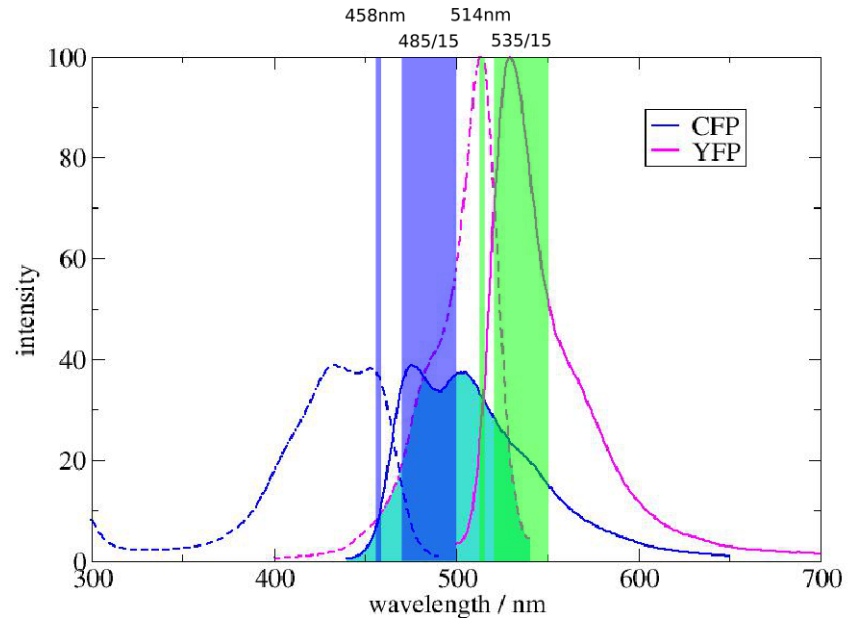
\includegraphics[width=0.4\textwidth]{FzV/Spektrum.png}
    \caption{Absorptions- und Emissionsspektrum der CFP/YFP Proteine}
\end{figure}\\
Wenn man nun Donor und Akzeptor tauschen würde, dann würde sich die Emissionslinie des neuen Donors (pink, durchgehen) nicht (bzw. nur knapp) mit der Absorptionslinie des neuen Akzeptors (blau, gestrichelt) schneiden.
Somit gibt es keinen FRET von Akzeptor zu Donor.
\section{Abstand für FRET}
\textbf{Welchen Abstand sollten PH-CFP und PH-YFP haben um FRET zu sehen?}\\
Der Abstand zwischen Donor und Akzeptor sollte in etwa dem Försterradius entsprechen.\\
Für die verwendeten Farbstoffe CFP und YFP liegt der Försterradius in der Größenordnung $5\,\text{nm}$ \citep[vgl.][]{foersterradius}.
\section{Crosstalk-Verunreinigung}
\textbf{Warum kann man nicht einfach den Donor anregen und schauen ob im Spektralbereich des Akzeptors Licht detektierbar ist? Worauf basieren eventuell nötige Korrekturen?}\\
Man kann die FRET-Intensität nicht direkt messen, da sich die Anregungsbereiche des Donors und Akzeptors teilweise überlappen.
Somit wird bei der Anregung des Donors auch der Akzeptor angeregt.
Wenn man nun nur die Emission des Akzeptors misst, ist diese 'verunreinigt' durch die partielle Anregung des Akzeptors.\\

Um dies zu bereinigen, misst man die Anregung des Donors und Akzeptors einzeln und kann somit die Crosstalk Beiträge berechnen.\newpage
